\documentclass{pracamgren}

%\usepackage{color}

\usepackage[T1]{fontenc}
\usepackage{lmodern}

\usepackage[table, svgnames, dvipsnames]{xcolor}
\usepackage{algpseudocode}
\usepackage{algorithm}
\usepackage[framemethod=tikz]{mdframed}
\usepackage{amsmath}
\usepackage{amsfonts}
\usepackage{epsfig}
\usepackage{pstricks}
\usepackage{graphicx}
\usepackage{algorithm}
\usepackage[backend=biber,style=authoryear-comp,sorting=nyt,maxcitenames=2,uniquename=false,uniquelist=false,maxbibnames=5,maxsortnames=1]{biblatex}
\usepackage[font=small,labelfont=bf]{caption}
\usepackage[hidelinks,allcolors=black]{hyperref}
\usepackage{upgreek} 
\usepackage{placeins}
\renewcommand{\arraystretch}{1.1}

\setlength{\parskip}{0pt}

\addbibresource{msc-thesis.bib}

\author{Maciej Manna}

\nralbumu{1065745}

\title{Massively Parallel Pseudo-Spectral DNS and~LES for Particle-Laden Turbulent Flows under Two-Way Momentum Coupling}

\tytul{Masywnie równoległe pseudo-spektralne symulacje DNS i LES przepływów turbulentnych z\,cząstkami przy uwzględnieniu dwustronnego sprzężenia pędu}

\kierunek{computer science}

\opiekun{Dr. hab. Bogdan Rosa \\
Warsaw University of Life Sciences -- SGGW \\
Institute of Information Technology; \\
Institute of Meteorology and Water Management \\ National Research Institute
}

\date{September 2022}

\keywords{obliczeniowa mechanika płynów, przepływ turbulentny, przepływ wielofazowy, krople, mikrofizyka chmur, obliczenia dużej mocy, równania Naviera-Stokesa, homogeniczna izotropowa turbulencja, statystyki zderzeniowe kropel, metoda pseudo-spektralna, bezpośrednia symulacja numeryczna (DNS), metoda dużych wirów (LES), dwustronne sprzeżenie pędu, efekty grawitacyjne}

\keywordsang{computational fluid mechanics, turbulent flow, multiphase flow, droplets, cloud microphysics, high performance computing, Navier-Stokes equations, homogeneous isotropic turbulence, droplet collision statistics, pseudo-spectral method, direct numerical simulation, large-eddy simulation, two-way momentum coupling, gravitational effects}


\begin{document}
\maketitle

\streszczenie{
Przepływy turbulentne z cząstkami fazy rozproszonej zachodzą nieustannie w środowisku naturalnym oraz znajdują liczne zastosowania w procesach przemysłowych.
Ważnym tego przykładem są chmury atmosferyczne, które składają się z ogromnej ilości małych kropel wody i kryształków lodu.
Wyjaśnienie wzajemnego oddziaływania powietrza (płynu) i aerozolu (cząstek) jest istotne w kontekście poznania mechanizmów rządzących powstawaniem i przebiegiem zjawisk atmosferycznych.
Wiedza w tym zakresie jest użyteczna w obszarze meteorologii i służy do opracowywania coraz to bardziej realistycznych modeli powstawania opadu z kropel chmurowych.
To z kolei prowadzi do podniesienia dokładności i sprawdzalności numerycznych prognoz pogody.
Jednym ze sposobów badania przepływów dyspersyjnych są symulacje numeryczne. 
\newline \indent
Powszechnie stosowanym do tego celu narzędziem, zapewniającym wysoką dokładność, są tzw. bezpośrednie symulacje numeryczne (direct numerical simulation, DNS). 
Za pomocą symulacji DNS można pozyskiwać statystyki zderzeniowe cząstek, które to są użyteczne jako parametry w modelach obejmujących większe skale przestrzenne.
Symulacje DNS są~jednak kosztowne obliczeniowo, co ogranicza ich stosowalność do siatek o średnich rozmiarach (${\sim 2048^3}$ węzłów -- przy współcześnie dostępnych zasobach obliczeniowych).
DNS nie pozwalają modelować turbulencji charakteryzowanej wyższymi liczbami Reynoldsa ($R_{\lambda} \sim 10^4$), czyli takiej która obserwowana jest w powietrzu atmosferycznym. \newline \indent
Metoda dużych wirów (large-eddy simulation, LES) stanowi alternatywę dla DNS.
W tej metodzie drobnoskalowa turbulencja nie jest bezpośrednio rozwiązywana, ale jest parametryzowana przy użyciu modelu podskalowego.
Umożliwia to modelowanie przepływów turbulentnych o większej liczbie Reynoldsa przy użyciu siatek o mniejszej liczbie węzłów.
Ograniczenie złożoności obliczeniowej odbywa się jednak kosztem mniejszej precyzji i fizycznej dokładności.
Niniejsza praca stanowi porównanie obu metod (DNS i LES), zarówno w kwestii fizycznej dokładności, jak i wydajności, skupiając się w szczególności na symulacjach z dwustronnym sprzężeniem pędu pomiędzy płynem i cząstkami. 
Zostało wykazane, że LES stanowi obiecującą odpowiedź na ograniczenia DNSu, pomimo pewnych niedokładności wynikających z filtrowania turbulencji w najmniejszych skalach.
Różnice te, w większości przypadków, stają się mniejsze, gdy uwzględni się dwustronne sprzężenie pędu, w szczególności dla cząstek poddanych działaniu grawitacji.
\newline \indent
Przeprowadzone zostały również analizy kosztów obliczeniowych obu metod.
Choć zastosowanie LES zapewnia ogromną oszczędność w obliczeniach związanych z turbulentnym przepływem płynu, to jednak koszt ten znacząco rośnie wraz z liczbą cząstek.
Niezbędna ilość symulowanych cząstek może zaś być duża, gdyż efekty dwustronnego sprzężenia pędu objawiają się wyraźniej w układach z względnie wysokim stosunkiem masy cząstek i płynu (pomiędzy $0.1$~i~$1$).
Obliczenia odnoszące się do dynamiki cząstek stanowią więc bardziej istotne ograniczenie dla LESu niż dla DNSu, gdzie złożoność obliczeń związanych z~płynem jest czynnikiem dominującym.
Ponadto zidentyfikowano i przeanalizowano szereg parametrów, które pośrednio wpływają na czas trwania symulacji, takie jak np. promienie kropel oraz~działanie grawitacji.
Na~koniec przedstawiono także wpływ preferencyjnego koncentrowania się cząstek na wariancję ich rozkładu pomiędzy równolegle wykonywanymi procesami.
Ten czynnik ma~również istotne znaczenie w kontekście całkowitej wydajności symulacji.
}

\renewcommand{\abstractname}{Abstract}
\begin{abstract}
Turbulent fluid flows with dispersed particles are a common occurrence in nature, as~well~as in many technological processes.
An important example of such systems are atmospheric clouds that consist of a huge number of small water droplets and ice crystals suspended in air.
The~understanding of interplay between air (fluid) and aerosol (particles) is crucial for increasing the accuracy and reliability of numerical weather forecasts through more realistic modelling of atmospheric phenomena.
Performing numerical simulations on a fine scale is one way of studying such processes.

Direct numerical simulations (DNS) prove to be a relatively precise tool that is widely used in these studies.
DNS can be used to obtain the particle collision statistics obtained from these simulations may be further utilised as parameterisations for larger-scale models.
These simulations, however, are costly in terms of computational complexity, hence their application is limited to moderate-sized grids ($\sim 2048^3$ nodes, with the computing power of modern supercomputers).
For that reason DNS are not able to resolve turbulence characterised by~higher Reynolds numbers ($R_{\lambda} \sim 10^4$), which is observed in atmospheric air.  

Large-eddy simulations (LES) provide an alternative approach to DNS.
In this method small-scale turbulence is not directly resolved but parameterised using a subgrid-scale model.
This reduces the grid size required to achieve higher Reynolds numbers (and, thus, computational complexity) at the cost of diminished precision and physical fidelity. 
This thesis provides comparison of DNS and LES, both in terms of physical fidelity and performance, focusing primarily on simulations under two-way momentum coupling between the fluid and particles.
LES is shown to be a promising solution to limitations of DNS, even though it~exhibits certain inaccuracies that may be attributed to the filtering of small-scale vortical structures.
These discrepancies, for the most part, become less pronounced when two-way momentum coupling is considered, especially for settling particles.

Furthermore, a broader study of computational costs for both methods is presented.
Even~though LES provides immense performance advantage when it comes to fluid simulation, it~is~highly susceptible to the growing number of individually tracked particles.
The amount of particles that are needed may be considerable, as effects of two-way momentum coupling manifest when particle mass loadings are relatively high (between $0.1$ and $1$).
Thus, computations related to particles are recognised to be a much more significant bottleneck for~LES than for DNS, where the complexity of fluid simulation is the largest concern.
In~addition, several parameters that indirectly influence the execution time are identified and analysed, such as droplet radii or effects of gravity.
Finally, it is shown that the preferential concentration of particles may affect the variance of their distribution between parallel processes and~consequently influence the overall simulation performance.
 
\end{abstract}


\tableofcontents


\chapter*{Acknowledgements}
\addcontentsline{toc}{chapter}{\numberline{}Acknowledgements}
\label{ch:ack}

This thesis was created as part of a project: \emph{Turbulent flow analysis with the dispersion phase -- the impact of two-sided coupling of momentum and gravity on particle motion statistics} of National Science Centre (NCN) -- OPUS14/2017, project no.: UMO-2017/27/B/ST8/00555.

The access to computational resources and supercomputer \emph{Okeanos} used to obtain results presented in this thesis was provided by Interdisciplinary Centre for Mathematical and Computational Modelling (ICM) at Warsaw University (grants: GA73-14, GA84-22, and G87-1145).

\medskip

First and foremost, I would like to thank the supervisor of this thesis and grants mentioned above, Dr. hab. Bogdan Rosa (Warsaw University of Life Sciences -- SGGW, Warsaw; Institute of Meteorology and Water Management -- National Research Institute, Warsaw), for excellent introduction and guidance in the subject matter of the thesis, as well as continuous encouragement and understanding during the process of its creation.
I would also like to express my gratitude to Dr. Sylwester Arabas (Jagiellonian University, Kraków), who introduced me to the modelling of atmospheric clouds and supported in pursuing further involvement in that field, for his valuable comments, as well as aid in administrative affairs.
Furthermore, I would like to acknowledge all creators, maintainers, and developers of the pseudo-spectral solver code, especially Prof. Lian-Ping Wang (University of Delaware; currently Southern University of Science and Technology, Shenzhen) and Dr. hab. Bogdan Rosa, as well as the copyright holder, University of Delaware, for permission to use and modify it in order to obtain results presented in this thesis.
Finally, I would like to thank Prof. Jacek Pozorski (Institute of Fluid Flow Machinery, Polish Academy of Sciences, Gdańsk), as well as all participants of A2S Group Seminar (AGH University of Science and Technology, Kraków) and Seminar on Partial Differential Equations (Jagiellonian University, Kraków) for valuable questions and discussions that helped in shaping the final draft of this thesis. 



\chapter*{Introduction}
\addcontentsline{toc}{chapter}{\numberline{}Introduction}
\label{ch:int}

Turbulence is the phenomenon that accompanies most of the real-world situations where fluid flows are encountered.
Distinction between laminar and turbulent flows is very practical, as the former represents much more organised, layered, and stable fluid motion that is easier to analyse and quantify, while the latter is inherently irregular, and its parameters have to be approached statistically.
Turbulence gives rise to eddies that span wide range of spatial and temporal scales where different dynamical properties of the fluid are most pronounced.
We commonly distinguish three subranges in the entire span of eddy sizes.
There is integral length scale that includes largest eddies containing most of the energy of a system.
Then, we consider inertial subrange, where turbulence kinetic energy is transferred from larger eddies to the smaller ones in a process referred to as the energy cascade.
Finally, we have subrange that consists of smallest eddy sizes, the so-called Kolmogorov microscale, where influence of fluid viscosity is paramount, and where the kinetic energy of slowly vanishing eddies is dissipated into heat.
Such complex behaviour arises due to the nonlinearity of equations governing the fluid motion, which makes turbulent flows famously difficult to study analytically.
Hence, numeric simulations are often employed to model and study these physical phenomena.

Many processes that involve fluid flows, whether laminar or turbulent, are composed of more than one phase.
Here, by phase, we understand regions of the system with the same properties that can be clearly separated by some interface from others.
We refer to such flows as multi-phase, or two-phase, in a common case where the number of considered phases is limited to two.
These phases often are of different states of matter, e.g. gas--liquid for air bubbles flowing in the water pipe, but systems with two immiscible liquids, such as water and crude oil in pipelines, are also studied \parencite{Brauner2003}.
In many cases, one of the phases may be treated as continuous (referred to as the continuous phase, or the carrier fluid), while the other remains in separated chunks.
We refer to such chunks as the disperse phase, and examples may include air bubbles, water droplets, solid particulate matter suspended in a fluid, etc.
Often enough, elements of disperse phase may be approximated as point particles, i.e. material points that are conceptually representing small spheres of given radii, that are considered insoluble and immiscible (that is, they cannot exchange mass with the carrier fluid, suddenly appear, or be destroyed).
Such approximation is especially accurate when disperse phase consists of small droplets or bubbles of one fluid surrounded by another, as the surface tension naturally preserves spherical shape of disperse elements.
Cloud droplets, in particular, remain spherical since the capillary pressure is several orders of magnitude larger than the local fluid shear stress induced by the disturbance flow associated with their motion.
Furthermore, \textcite[Figure 1, therein]{Balachandar2010} point out that for such approximation to be valid, particle response times have to be greater than Kolmogorov time scale of background turbulent flow. 
We shall refer to two-phase flows with disperse phase approximated by point particles as particle-laden.

The modelling of flows that both exhibit turbulent behaviour and include population of particles interacting with that flow gives rise to even more complexity.
As stated by \textcite{Balachandar2010}, ``turbulence and multiphase flows are two of the most challenging topics in fluid mechanics, and when combined they pose a formidable challenge, even in the dilute dispersed regime''.
In spite of that, the number and importance of real-life applications that involve such systems is quite significant, and more than justifies development of effective methods in that domain.
To mention just a few, we may consider some technological, and industrial applications, such as analysis of combustion of liquid fuel aerosols in engines, or combustion of pulverised coal in furnaces \parencite{Zheng2020}, as well as other technologies, including fluidised beds, transport systems, and pollution control \parencite[4-17]{Crowe2012}.
Such systems are also studied in ecology (e.g. transport of pollutants in the atmosphere or sediments in water) and agriculture (efficient spraying of fertilisers).
Finally, the modelling of atmospheric clouds, that essentially are huge collections of small water droplets and ice crystals suspended in often turbulent air, is the backbone of all meteorological and climate science models used for analysis and prediction \parencite{Devenish2012, Grabowski2013}.
In this thesis we shall focus our study of particle-laden turbulent flows on applications in cloud modelling, but general methods presented here are not limited to that particular use case.

The modelling of atmospheric clouds is a broad domain that has to deal with wide range of length scales, where different structures and physical processes are important and have to be directly represented, while others need to be parameterised due to constraints in computing power.
Such tradeoff between computational complexity and physical fidelity of simulations gives rise to the plethora of methods used depending on the respective scale.
Simplified picture of that situation is presented in Figure \ref{fig:atmo-scales}.
At the largest scales we have global climate models (GCM) and global weather models (GWM, e.g. Integrated Forecasting System, Global Forecasting Systems, ICON), where computation domain  often spans the entire Earth ($\sim 10^{7}$~m) and each cell has (horizontal) dimensions ranging from $10$ to $100$ kilometres.
We also consider mesoscale models that are mainly used for weather prediction in smaller domains that usually cover regions, countries, or continents ($\sim 10^{5} \text{--} 10^{6}$ m) and grid spacing is in the order of kilometres.
For instance, maximal resolution of mesoscale model COSMO used for weather forecasting in Poland is $2.8$ km \parencite{Doms2021}.
In this context it is worth adding that a small cloud with a volume of $1 \; \text{km}^3$ may contain $10^{17}$ or more droplets.
Both types of models, due to relatively large grid cell sizes, cannot fully resolve even fairly large cloud structures and depend on a lot of parameterisations.
In the middle ground, we have cloud resolving models (CRM; domain sizes---kilometres, cell sizes---metres) that cannot fully resolve all turbulent scales of air or exactly model behaviour of every droplet, thus necessary parameterisations are employed, such as large-eddy simulations (LES) and super-droplet method \parencite{Arabas2013}.
CRM is commonly employed for research studies focused on the effects of microphysical processes affecting entire clouds, their formation and evolution, precipitation, etc.
For that reason, CRMs are used to refine cloud parameterisations used in GCM and mesoscale models.

\begin{figure}[h]
\centering
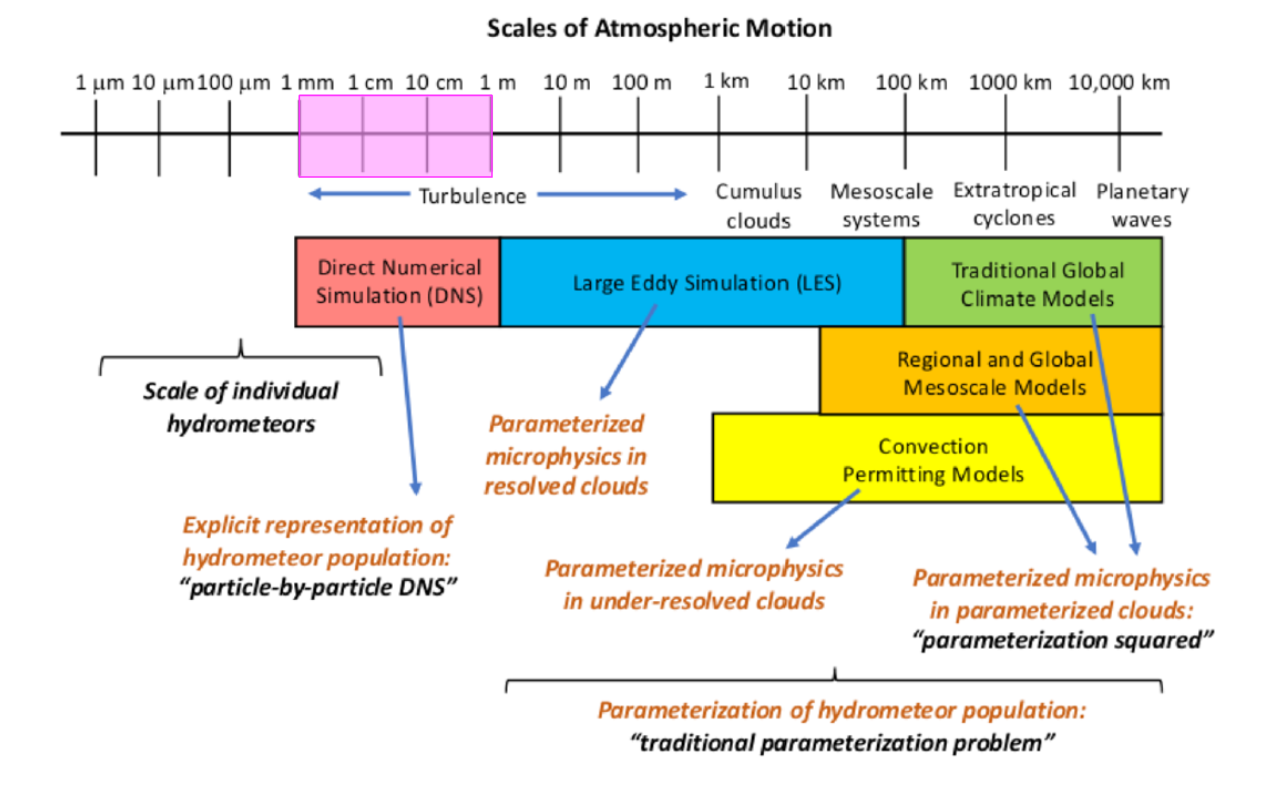
\includegraphics[width=13cm]{figures/0-01_atmo-scales.png}
\caption{
Hierarchy of atmospheric models and the scales of atmospheric motion reproduced from \textcite{Morrison2020} with author's permission.
Coloured rectangles represent types of simulations commonly used when working with respective length scales, and comments emphasise transition from directly resolving most elements of the model (left) to including more and more parameterisations with the increase of scale (right).
Magenta rectangle positioned on the axis was added to emphasise range of scales that corresponds to simulations discussed in this thesis.
}
\label{fig:atmo-scales}
\end{figure}

Finally, we enter scales where point-particle direct numerical simulations (DNS) can be used to obtain more precise picture of small-scale turbulent phenomena that affect cloud microphysics.
These methods allow direct resolution of wide range of turbulent scales, including Kolmogorov microscales, which are estimated to be of the order of 1 mm in Earth's atmosphere.
Also, all particles (droplets) are individually tracked, so that their dynamics and interaction with carrier flow may be directly computed (note, that $1 \, \text{m}^{3}$ of cloudy volume contains, approximately, up to $10^{8}$ droplets).
Due to fine sizes of grid cells required to resolve even the smallest eddies, as well as considerable computational demand of handling large numbers of particles, point-particle DNS are limited to volumes of about $1 \, \text{m}^{3}$ \parencite{Morrison2020}.

Despite these limitations, however, such simulations provide essential backbone to entire hierarchy of models by allowing to study small-scale cloud phenomena and estimate parameters used in cloud resolving models (CRM).
One example of such parameter is the collision kernel that determines rates of collision between droplets of the same or different sizes, and it greatly affects process of droplet growth due to coalescence that is crucial for accurate modelling of precipitation.
Such small domains also justify modelling air turbulence as homogeneous and isotropic.
Even though energy-containing large-scale eddies in atmosphere generate large-scale inhomogeneity and anisotropy, dissipative small-scale eddies work to flatten the inhomogeneities, leading to local homogeneity and isotropy.
This local homogeneity assumption is the basis of most turbulence models \parencite{Matsuda2021}.

There is, however, another important axis which exhibits similar complexity--fidelity tradeoff, and it pertains to the precision of modelling interactions between particles and carrier fluid.
We use Lagrangian approach to track particles, since time microscales associated with the energy dissipation of atmospheric flows and response times of cloud droplets are usually of the same order (i.e. the Stokes number, $St$, is close to $1$, see \cite{Balachandar2009}).
The modelling of interaction between fluid and particles, however, may be limited to one-way momentum coupling (OWC).
It means that particles are transported by the fluid but do not affect its velocity field.
This simplification is valid for dilute systems, where ratio of total mass of particles to total mass of fluid (referred to as the particle mass loading, $\Phi_m$, of the system) is small, usually assumed to be less than $0.1$ (i.e. less than $0.01\%$ by volume for water droplets in air).
Despite that, experiments have shown that presence of particles alters statistics of the carrier fluid flow, e.g. suppresses or enhances the turbulence flow depending on the sizes of particles \parencite{Gore1989}.
Also, recent simulation studies \parencite{Rosa2020} have shown that inclusion of momentum transfer in the other direction, i.e. two-way momentum coupling (TWC), provides a more complete and complex picture of system dynamics, and increase physical fidelity of obtained results, even for relatively dilute systems.
Hence, TWC approach is used here, building upon methods and results from \textcite{Rosa2020,Rosa2022}.
Note, that for very dense systems ($\Phi_m > 1$) it is preferable to also include effects of collisions between particles (four-way momentum coupling), but such conditions are not applicable when considering Earth's atmospheric clouds.
Also, in this context, it is worth to mention alternative methods for modelling interactions between particles, such as simplified representation of many-body aerodynamic interactions \parencite[Hybrid DNS, see][]{Wang2009, Ayala2007} or inclusion of lubrication forces \parencite{Ababaei2021}, however these approaches are beyond the scope of this study.

\smallskip

In this thesis, small-scale simulations of turbulent, particle-laden flows are considered for the purpose of obtaining particle collision statistics, such as previously mentioned collision kernels.
The domain in question is small enough that we can employ direct numerical simulations for the modelling of homogeneous isotropic turbulence (HIT).
For simplicity, the domain is assumed to be box-shaped and uniformly divided into cubic cells in all three dimensions.
Also, periodic boundary conditions are imposed on the domain walls.
As introduced above, the default method applicable for such experiments is point-particle DNS.

Recent studies, however, have shown that direct numerical simulations are close to their limits due to prohibitively large computational costs.
\textcite{Rosa2013,Rosa2016} used grids of up to $1024^3$ nodes, which seems to be the reasonable limit for most studies, although there were studies using even larger grids---e.g. $2048^3$ nodes in \textcite{Ireland2016} and \textcite{Matsuda2021}; for flows without particles grids of size $8192^3$ were used \parencite{Buaria2019} and more recently even up to $12\,288^{3}$ \parencite{Buaria2020}.
It is important to note that grid size is crucial for turbulent flow simulations since it affects the range of spatial scales that can be resolved---from the smallest eddies with sizes close to the spatial grid spacing, to the largest ones of sizes typically about $1/3$ of the computational domain (this limitation is due to a numerical requirement that the correlation of fluid velocity at distances comparable to the domain size must vanish).
Such range between largest and smallest resolvable scales can be expressed using Reynolds numbe, which is commonly interpreted as a measure of magnitude of turbuence.
Examples of values of the Taylor microscale (that is, considering only eddies in inertial subrange) Reynolds number, $R_{\lambda}$, attained in previous high-resolution studies are $R_{\lambda} = 499$ for $1024^3$ grid \parencite{Rosa2013,Rosa2016}; $R_{\lambda} = 597$ \parencite{Ireland2016}, and $R_{\lambda} = 531$ \parencite{Matsuda2021} for $2048^3$ grids; $R_{\lambda} = 650$ for $8192^3$ \parencite{Buaria2019}; and $R_{\lambda} = 1300$ for $12\,288^3$ grid.
It is desirable, however, to attain higher values of $R_{\lambda}$ to simulate conditions that are present in typical atmospheric clouds, where $R_{\lambda}$ is known to attain values between $10^{3}$ and $10^{4}$.
What is more, the increase of the Taylor microscale Reynolds number with the number of grid nodes in one dimension, $N$, is sublinear (comparison of simulation data from various studies shows that $R_{\lambda} \propto N^{2/3}$, see \cite{Wang2009}, Figure 1 therein, which agrees with theoretical estimates for pseudo-spectral method in \cite{Pope2000}, Equation 9.8 therein).
Thus, when we double $N$ we only increase $R_{\lambda}$ by at most $50\% \text{--} 60\%$, while total number of grid nodes, $N^3$, increases by the factor of $8$.
The strategy of increasing grid sizes of DNS to model somewhat wider range of turbulent scales currently faces not only resource limitations, but is also hindered by the diminishing returns in the long run.
This situation calls for an alternative solution.

Large-eddy simulation (LES) is a well-developed method that is commonly used when dealing with length scales specific to CRM simulations \parencite{Guichard2017}.
Its purpose is to allow modelling of highly turbulent environments in larger domains, where directly resolving smallest eddies is infeasible.
The general idea is to directly resolve larger eddies, as in DNS, but replace the direct resolution of the smallest, dissipative turbulent scales with parameterised model, referred to as the subgrid-scale model.
This way smaller grid sizes may be used to obtain statistics of turbulent flow that are comparable to DNS, including the Reynolds number.

LES focuses on directly resolving larger scales of turbulence since they contain most of the energy of the system, and are most effective transporters of conserved properties (\cite[367]{Ferziger2020}; \cite[352]{Pope2000}).
This property is paramount for CRM, but when using simulations to study small-scale phenomena such strategy is not as easily transferable.
Also, it was repeatedly shown that relative motion and preferential concentration of low-inertia particles is governed mainly by small turbulent structures.
Consequently, the collision-coalescence depends on scales of motion that belong to the dissipation subrange of the energy spectrum.
The interest in applying LES method in small-scale experiments used to estimate particle statistics may be limited, but is growing in recent decades \parencite{Fede2006, Jin2010, Rosa2017}, but no comparable studies that also include effects of TWC were performed.
Therefore, it is called for to investigate feasibility of LES in that context, and this thesis aims at providing good starting point for such analyses.

\medskip

The first systematic study using DNS of homogeneous and isotropic turbulence with non-settling particles (i.e. unaffected by gravity) under two-way momentum coupling was performed more than thirty years ago by \textcite{Squires1990}.
It focused on the effects that particles have on carrier flow, especially the modulation of turbulence and changes in energy and dissipation spectra due to varying particle mass loadings.
Their simulations, due to contemporaneous hardware limitations, used small grid sizes ($32^3$ and $64^3$) and thus were limited to $R_{\lambda} = 38$.
In a follow-up study by \textcite{Elghobashi1993} the effect of gravitational settling was considered but the simulations were limited to decaying turbulence.
Other early studies, such as \textcite{Wang1993} and \textcite{Yang1998}, expanded these results to larger meshes but were limited to the one-way momentum coupling.
More importantly, the latter study \parencite{Yang1998} proposed to use LES to achieve higher $R_{\lambda}$ without going beyond hardware limitations.

These earlier studies, however, did not explicitly consider collisional statistics of particles, such as collision kernels, which are main focus of this thesis.
One of the first systematic studies aimed at estimating these parameters using DNS with homogeneous isotropic turbulence model was \textcite{Ayala2008}, and it was motivated by growing interest in the process of droplet growth due to collision-coalescence.
Their simulations included effects of gravity and were performed at different values of the energy dissipation rate.
In another study by \textcite{Wang2008} the main focus was also on collision statistics, but also hydrodynamic interaction between droplets was considered by employing an original method elaborated by \textcite{Ayala2007}.
In both cases, no influence of particles on the fluid flow was taken into account (as in TWC), but their method attempted to model hydrodynamic interactions between particles instead.
An example of earlier TWC study that focused on  particle statistics may be the work of \textcite{Bosse2006}, that shows significant enhancement in the mean settling velocity when two-way coupling is considered. 
Later, these results were extended by \textcite{Monchaux2017} for wider ranges of particle volume loadings, also reporting decrease in particle preferential concentration with increasing mass loading.

Two important features of further studies, at least from the point of view of this thesis, are: (1) inclusion of two-way momentum coupling between fluid and particles, and (2) use of large-eddy simulations in that context.
Most of these, however, used only direct numerical simulations that were limited to one-way momentum coupling.
\textcite{Rosa2013} provides results from simulations spanning wide range of grid sizes (from $N=32$ to $N=1024$), and shows, in practice, diminishing growth of $R_{\lambda}$ with respect to $N$.
It also analysed the influence of different forcing schemes on the estimated particle statistics.
Further studies by \textcite{Onishi2013} and \textcite{Ireland2016} are notable because of relatively large grids used that allowed to obtain higher values of $R_{\lambda}$ ($N=2048$ with $R_{\lambda}=597$, and $N=2000$ with $R_{\lambda} = 527$, respectively).
Work by \textcite{Onishi2013} is also worth mentioning, as instead of pseudo-spectral method it uses finite-difference method, which is considered to be easier to parallelise and adapt to multiprocessor machines.
On that note, of some interest are also recent papers that use Lattice Boltzmann Method to solve underlying homogeneous and isotropic turbulent flow populated by particles tracked using Lagrangian approach \parencite{Ernst2019,Lain2020}.
These studies, however, used only grids of size $128^3$ and since working with highly turbulent flows was not their main goal they were limited to $R_{\lambda} = 20$.
More recent study of \textcite{Matsuda2021} is notable for used grid sizes (up to $2048^3$) and impressive number of particles tracked (up to $1$ billion), as well as interesting measurements of scale-dependent flatness and skewness of particle distribution fields based on wavelets.
Still, these experiments were limited to one-way momentum coupling.

Nonetheless, as already mentioned, it was recent study of \textcite{Rosa2020} that systematically analysed the effects of including two-way momentum coupling on basic statistics of the carrier flow, as well as collision statistics of particles.
Their results show that using TWC significantly affects particle statistics that measure clustering, radial relative velocities, and collision rates, as well as dependence of these statistics on the particle mass loading.
These results were recently complemented by \textcite{Rosa2022}, where simulations covering broader range of grid sizes were performed (up to $1024^3$), and the influence of TWC on average settling velocity of particles was explored as well. 
Still, both of those studies were limited to DNS method only.

On the other hand, first systematic study of using LES method for simulating steady homogeneous isotropic turbulence for carrier fluid in particle-laden systems was performed by \textcite{Fede2006}.
Simulations were performed using finite-volume method on grids with $128^3$ nodes.
Their effort was focused on measuring influence of subgid-scale modelling on the behaviour of heavy inertial particles at collision distances.
In particular, they established that using LES significantly affects particle concentration and collision statistics, as they depend on small-scale motion of carrier fluid.
Their analysis was limited to non-settling particles.
\textcite{Marchioli2008} arrived at similar conclusions, i.e. that filtering velocity field at small-scales leads to inaccuracies in representation of particle segregation and accumulation phenomena in simulations involving wall-bounded flows.
Meanwhile, \textcite{Yang2008} showed that for different particle statistics, such as longtime single-particle dispersion, some effects of LES parameterisation cancel each other, leading to accurate predictions.
More in depth study on the influence of subgrid-scale modelling on preferential concentration of particles, where principal requirements for such models were established, was proposed by \textcite{Pozorski2009}.

Important comprehensive study of impact of subgrid-scale modelling on particle collision statistics in HIT was performed by \textcite{Jin2010}.
They used the pseudo-spectral method for the fluid flow calculations and their realisation of LES (i.e. using spectral eddy viscosity model) matches numerical method used in this thesis.
Their results confirmed adverse effect of LES on the accuracy of particle-pair statistics, as well as established relation between Stokes number, $St$, and sensitivity of these statistics to subgrid-scale modelling.
They concluded that such effects are most noticeable when $St < 3$.
This study involved only non-settling particles.
It was later complemented by \textcite{Rosa2017} that used the same numerical setup but focused on particles affected by gravity.
Their results confirmed previous conclusions regarding limitations of LES to properly represent collisional statistics, such as radial distribution function and radial relative velocity.
They also established influence of subgrid-scale modelling on seemingly single-particle statistics, such as average settling velocity.
All studies mentioned above were limited to one-way momentum coupling.

\smallskip

The natural continuation of aforementioned studies is to analyse the influence of both such extensions applied together in the same simulations.
Thus, more precisely, the topic of this thesis regards simulations of homogeneous isotropic turbulence with inertial particles under two-way momentum coupling, both with and without effects of gravity, for the purpose of estimating their collisional statistics.
Also effects of particles on basic flow statistics shall be discussed.
Both direct numerical simulations (DNS) and large-eddy simulations (LES) are used to obtain results, providing grounds for comparison of both methods.
To the knowledge of the author, it is the first study in this context, where TWC LES simulations are considered.
For the sake of simplicity, all simulations performed as part of this study will use single, moderately-sized grid of $256^3$ nodes for DNS, and $64^3$ for LES, as in \textcite{Jin2010} and \textcite{Rosa2017}.
This study aims to fit into much broader and pressing issue of computational limits that are faced by DNS and establishment of LES as an alternative that opens way to more faithful modelling of atmospheric turbulence.

\smallskip

The comparison between DNS and LES is carried out in two following aspects.

Firstly, the accuracy, or physical fidelity, of LES is analysed.
Establishing exact measures of accuracy for collisional statistics is a challenging task because of experimental constraints, as simultaneous measurement of positions and velocities of large amounts of small droplets faces technical limitations, although considerable advances have been made recently in that field \parencite{Yavuz2018}.
Moreover, homogeneous and isotropic model of turbulence is an idealisation that could not be exactly replicated in actual physical conditions.
For these reasons it is difficult to obtain experimental results for validation, and due to the complexity of the problem at hand, no analytical solutions are available as well.
On the other hand, difficulties in obtaining experimental data makes estimations of these statistics \emph{in silico} even more valuable.
Thus, as in previous studies, the accuracy comparison will mostly focus on qualitative and quantitative differences between results obtained by DNS and LES.
The results of DNS are used as a baseline, under the assumption that this method is thoroughly studied and frequently used, and thus provides accurate estimates of parameters in question.
Hence, results obtained using LES are compared against them, in order to consider feasibility of LES as a workable replacement for DNS.
The further analysis will focus mainly on simulations under two-way momentum coupling.

Secondly, the performance of these two methods will be compared.
The main advantage of LES is its reduced computational cost while attaining similar values of $R_{\lambda}$.
Such claim needs to be thoroughly verified, especially when simulations with particle-laden flows are considered, where computational load not only scales with grid size used to resolve fluid flow but also with the number of individually tracked particles.
That impact is not easy to predict as computations concerning both phases are performed side-by-side in a massively parallel context.
Thus, a series of experiments will be performed to establish possible performance gains provided by LES and whether they can be easily achieved by using the same code architecture and parallelisation strategy as for DNS.

The organisation of this thesis directly follows goals and aspects of analysis outlined above.
The entire text is divided into three chapters.
The first one consists of brief explanation of the numerical method underlining all simulations used to obtain results presented thereafter.
The emphasis is placed on the pseudo-spectral method used for fluid flow simulation, difference between DNS and LES methods, and modelling of interactions between fluid and particles.
In addition, some information on implementation details is given.
Second chapter introduces relevant flow and particle statistics that are being estimated in simulations.
More importantly, the results of simulations will be presented and analysed here in order to compare the physical fidelity and feasibility of LES vs DNS.
Results related to modelling under one-way momentum coupling will be recreated, and validated with respect to previous studies.
Then, results that include the effect of two-way coupling will be presented for both DNS and LES, depending on particle radii, as well as particle mass loading.
In the last chapter, results of performance comparison between DNS and LES shall be presented and discussed.
These will focus on simulation wall-clock times depending on the various parameters of simulations, in order to estimate their influence on the computational cost of the solver code.
Also, more in-depth profiling data shall be presented, as well as analysis of particle distribution in computational subdomains and its impact on the performance of both methods.



\chapter{Numerical Methods}
\label{ch:ch1}

The challenges of numerical modelling of particle-laden turbulent flows are manifold and are mainly associated with the need to keep track of evolution of two distinct phases---continuous fluid flow and discrete particles---as well as their interactions.
In this study, the standard Eulerian-Lagrangian approach is used.
It introduces two different representations for two phases: velocity field of turbulent flow is evaluated on the nodes of a fixed grid, while each particle has its current position and velocity individually tracked.
Moreover, two different methods of simulating fluid flow are employed: direct numerical simulations (DNS) and large-eddy simulations (LES), both within the base framework of the pseudo-spectral method.
Finally, beyond conceptual and numerical issues, such multiphase systems prove difficult to be effectively implemented for a massively parallel computing environments (supercomputers) and it will be addressed in the last section.


\section{Fluid Flow Simulation with Pseudo-Spectral Method}
\label{sc:ch1.pspec}

The time evolution of turbulent fluid flow for simulations presented here is performed on the three-dimensional uniform cubical mesh with $N$ equally spaced grid points in each spatial dimension (see Figure \ref{fig:dns-les-grids}).
For this study, the domain size (for DNS) was set to $N=256$, for the total of $256^3 \approx 16.8$ million grid points.
The values of three-dimensional fluid velocity field $\mathbf{U}(\mathbf{x}, t)$ are evaluated at each time step and spatial grid point according to time-dependent Navier-Stokes equations for incompressible flows, as presented below in rotational form
\begin{equation}
  \left\{
  \begin{array}{ll}
  \frac{\partial \mathbf{U}}{\partial t} = - \mathbf{U} \times \boldsymbol{\omega} - \nabla \left( \frac{P}{\rho} + \frac{1}{2} \mathbf{U}^2 \right) + \nu \nabla^{2} \mathbf{U} + \mathbf{f} + \mathbf{f}^{(p)}\\
  \nabla \cdot \mathbf{U} = 0
  \end{array}
  \right.
  \label{eqn:n-s}
\end{equation}
where: $\boldsymbol{\omega} = \nabla \times \mathbf{U}$ denotes vorticity, $P$ -- pressure, $\rho$ -- fluid density, and $\nu$ -- kinematic viscosity of the fluid.
Other contributions come from large-scale force, $\mathbf{f}$, used to achieve and maintain the statistically stationary state of homogeneous isotropic turbulence, together with the cumulative force exerted by particles on fluid per unit mass, $\mathbf{f}^{(p)}$, which is non-zero for simulations under two-way momentum coupling (TWC) where effects of particles on the fluid flow are considered (see Section \ref{sc:ch1.part}).
Due to idealised nature of considered system, we may assume periodic boundary conditions in all three spatial directions.

The numerical integration of the Navier-Stokes equations is performed using the -spectral method which is well-established for such simulations.
It was first introduced by \textcite{Orszag1972} and later developed with parallel execution in mind and for application to particle-laden flows (e.g. see \textcite{Wang1993,Ayala2014,Parishani2015}).
It involves transformations of the velocity field between its representations in physical space, $\textbf{U}(\textbf{x}, t)$, and spectral (Fourier) space, $\hat{\textbf{U}}(\textbf{k}, t)$, in order to perform some operations in the space that is most favourable.
Detailed description of that method may be found in Appendix \ref{app:psm}.
Note, that performing Fourier transforms (implemented as FFT) is the most computationally demanding part of the method.
In the version of pseudo-spectral method used here, every iteration requires three 3D FFTs (1 forward and 2 inverse) for each component of the considered vector quantity and they dominate theoretical time complexity of the method, which is of order $N^3 \log N^3$ (per time step).

In the context of this study, pseudo-spectral method proves to be particularly effective method.
Due to its use of spectral space and Fourier transforms it allows to easily incorporate large-scale forcing required to maintain homogeneous isotropic turbulence.
For the same reason, it is also well-suited to be used with LES method, especially in a form that is proposed in this study (see Section \ref{sc:ch1.les}), since velocity field filtering is defined in terms of convolution operation that becomes trivial to apply in Fourier space.
Moreover, Fourier transforms that are repeatedly applied to fluid velocity field are consistent with periodic boundary conditions.
Also, even though the velocity field is mainly integrated in the spectral space, it is also transferred back to the physical space (as opposed to purely spectral methods) and can be further used to calculate interactions between fluid flow and particles localised by their physical coordinates.
Finally, pseudo-spectral method is known for its stability (if Courant-Friedrichs-Lewy number does not exceed 0.3) and superior computational accuracy for homogeneous isotropic turbulence \parencite{Peng2009}.
On the other hand, frequent use of Fourier transforms makes it difficult to be effectively implemented for massively parallel execution, as such operations require global access to data across computational subdomains.
Such overheads for data transfer between processes rapidly increase with grid size, therefore it is important to find methods of reducing grid sizes as pseudo-spectral method does not seem to scale well performance-wise beyond grids of size $N=1024$.

\medskip

The context of simulations studied here requires steady homogeneous isotropic turbulence to be maintained throughout the entire computation.
For that reason energy must be provided to the system in an adequate manner to make up for the losses due to dissipation inherent in  turbulent processes and sustain statistically stationary flow that exhibits desired characteristics.
Two main forcing schemes employed for that purpose are referred to as deterministic \parencite{Sullivan1994} and stochastic \parencite{Eswaran1988}. 
The effects of using both schemes on particle statistics (in OWC context only) were studied in \textcite{Rosa2011,Rosa2013,Rosa2015,Parishani2015}.
Slightly increased particle clustering and collision kernel values were observed with deterministic scheme, yet these discrepancies were deemed to be negligible, at least for the water droplets with radius smaller than $30$~$\upmu\text{m}$.
Also, most discrepancies attributed to the choice of forcing scheme manifest when simulation time scale is correlated with forcing, which is partly alleviated by using time step, $\Delta t$, that is relatively small with respect to Kolmogorov time scale of turbulence, $\tau_k$, as prescribed in \textcite{Rosa2015} (here, $\Delta t / \tau_k \sim 10^{-2}$).
Deterministic scheme, however, if properly parameterised, allows to achieve higher Reynolds numbers, $R_{\lambda}$, than by using stochastic forcing and this difference is important in this study.
Hence, simulations performed here use only deterministic forcing scheme.

\begin{figure}[h]
\centering
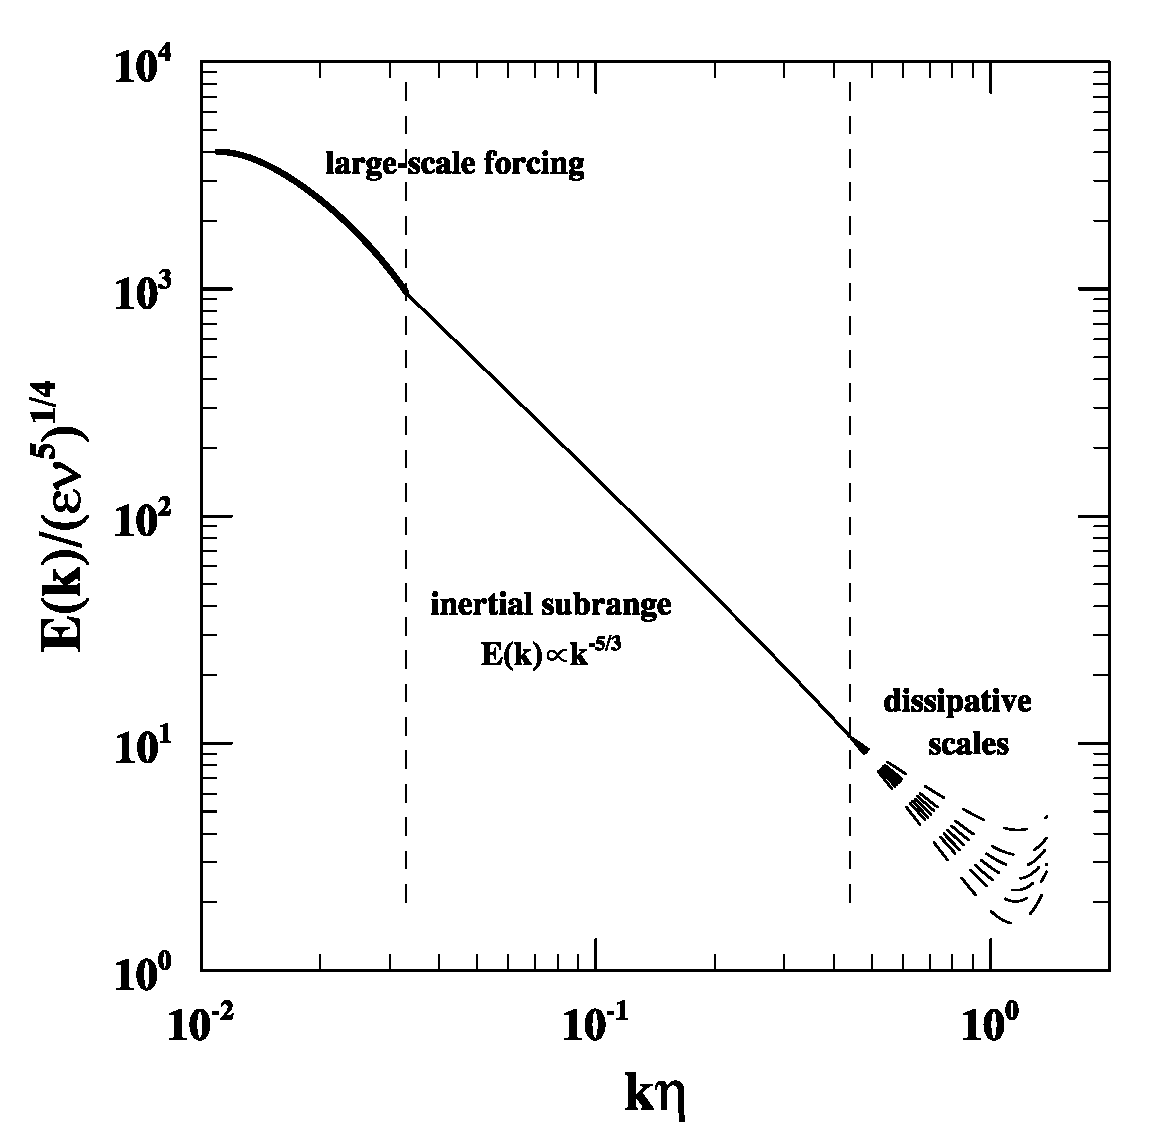
\includegraphics[width=10cm]{figures/1-01_forcing.pdf}
\caption{
The basic idea of deterministic forcing scheme: energy is supplied on large scales by fixing it for small wavenumbers (bold line), then it is transferred following Kolmogorov energy cascade ($E(k) \propto k^{-5/3}$) in inertial subrange, to finally reach smallest dissipative eddies represented by largest resolved wavenumbers (when $k_{\max} \eta \sim 1 = 10^0$, diverging dashed lines) that have largest influence on measured particle statistics at contact distances.
Both axes are using standard normalisations (see Section \ref{ssc:ch2.flow.spec}) and logarithmic scale, that makes $k^{-5/3}$ curves appear as straight lines.}
\label{fig:forcing}
\end{figure}

The basic idea behind deterministic forcing scheme, as laid out in \textcite{Sullivan1994}, is to set energy associated with largest eddies---or, equivalently, with lowest wavenumbers in the spectral space---to predetermined values in every time step.
In order not to affect the entire flow this is done only for very few wavenumbers ($|k| \in \{ 1, 2 \}$ in this study).
Then, due to energy cascade that characterises inertial scales of turbulence, the energy injected at low wavenumbers is transferred to the higher ones allowing to achieve statistically stationary state with desired characteristics of homogeneous isotropic turbulence (see Figure \ref{fig:forcing}).
It is accomplished by balancing large-scale energy input provided by the forcing term and energy depletion due to viscous dissipation at small scales. 
In case of this study, the contribution from the deterministic forcing, $\hat{\mathbf{f}}$, is included in Navier-Stokes equations in spectral space (see Equation \ref{eqn:mom-spec} in Appendix A, that is a Fourier-transformed version of Equations \ref{eqn:n-s}).
Here, following the setup used in \textcite[p. 6]{Rosa2011}, the values for 3D shells associated with two lowest wavenumbers ($0.5 < |\textbf{k}| < 1.5$ and $1.5 < |\textbf{k}| < 2.5$) are set to $0.555440$ and $0.159843$ (following Kolmogorov's $E(k) \propto k^{-5/3}$ spectrum), respectively.
For the remaining wavenumbers, $\hat{\mathbf{f}} = 0$, thus any smaller scales are not directly affected by forcing term.

\section{Large-Eddy Simulations}
\label{sc:ch1.les}

The pseudo-spectral method, as described above, is used in DNS to directly calculate the velocity field of turbulent flow for all grid nodes.
Despite important advantages, this method faces huge challenges in implementation for massively parallel execution \parencite{Onishi2013}. 
Moreover, when applied to DNS it faces problematic limitations in computational performance and scalability. 
Therefore an alternative approach is proposed, so called large-eddy simulation (LES). 
The main goal is to reduce the size of computational grid without losing ability to model systems with similar range of turbulent scales, as measured by Taylor microscale Reynolds number, $R_{\lambda}$.
This is achieved by directly resolving turbulent flow only for large and intermediate scales and replacing direct resolution of small-scale turbulence (as it is done in DNS) with one of the proposed models of turbulence, referred to as subgrid-scale (SGS) model.
Since we are replacing direct resolution with parameterisation, it is expected that the fidelity of results obtained using LES (when compared with DNS) may be diminished and they may be highly sensitive to the appropriate choice of the subgrid-scale model.
On the other hand, this allows a significant reduction in the size of used grid and, consequently, either increase computational performance of current simulations or enable new ones that achieve much higher $R_{\lambda}$.
This is possible because large part of computational effort in DNS is dedicated to resolving smallest turbulent scales \parencite[p. 558]{Pope2000}.
In case of this study, we use $N=64$ for LES and $N=256$ for DNS, thus the total number of grid nodes where fluid velocity field is directly resolved is reduced by the factor of $64$ (while still achieving comparable values of $R_{\lambda}$).
Conceptually, we may consider that each LES cell encompasses $4^3=64$ DNS cells where small-scale variations in velocity field would be directly resolved by integrating Navier-Stokes equations (see Figure \ref{fig:dns-les-grids}).

\begin{figure}[h]
\centering
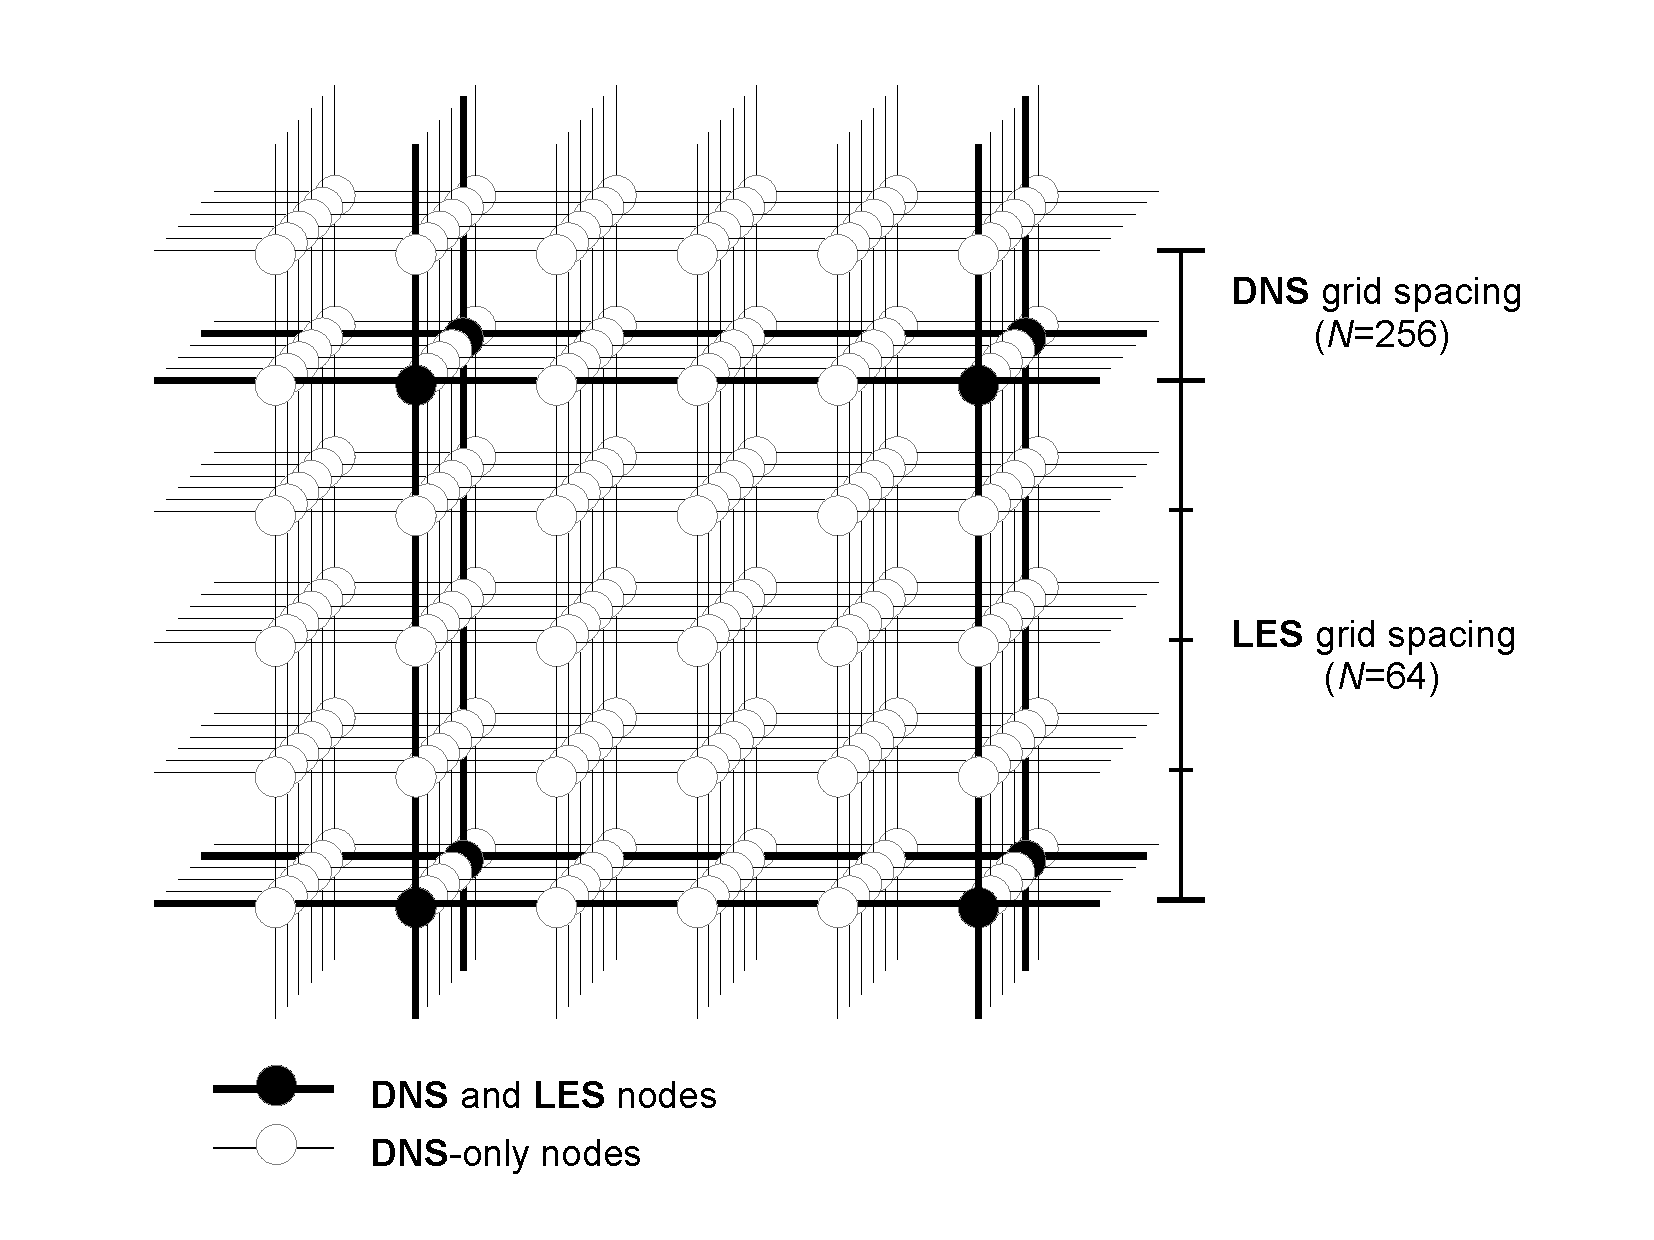
\includegraphics[width=17cm]{figures/1-02_dns-les-grids.pdf}
\caption{
Conceptual juxtaposition of computational grids for DNS and LES.
In LES, the subgrid-scale modelling parameterises small-scale turbulence that is directly resolved by $4 \times 4 \times 4$ block of cells in DNS.
}
\label{fig:dns-les-grids}
\end{figure}

In this study, that may be considered the continuation of \textcite{Rosa2017}, a similar setup for LES method is employed \parencite[based on earlier work by][]{Jin2010}.
In particular, the closure of the subgrid term is based on the concept of the spectral-eddy viscosity, $\nu_{e}$.
In spectral space, thefiltered velocity field $\hat{\bar{\mathbf{U}}}(\mathbf{k}, t)$ is governed by the following momentum equation \parencite{Pope2000}
\begin{equation}
\left\lbrace \frac{\partial}{\partial t} + [\nu + \nu_{e}(k|k_{c})]k^{2} \right\rbrace \hat{\bar{\mathbf{U}}}(\mathbf{k}, t) = \mathbf{P}(\mathbf{k}) \mathcal{F}(\bar{\mathbf{U}} \times \bar{\boldsymbol{\omega}}) + \hat{\mathbf{f}}(\mathbf{k}, t) ,
\label{eqn:les}
\end{equation}
where $\mathbf{P} \equiv \left\{ \mathbf{P}_{ij} \right\}$ is the projection tensor (see Equation \ref{eqn:proj-tensor}) and $\mathcal{F}$ -- Fourier transform.
By $k_{c}$ we denote cutoff wavenumber for filtering and its value is set using the same formula as maximal resolved wavenumber, $k_{\max}$, in DNS, i.e. $k_c = \left\lfloor (N - 3) / 2 \right\rfloor$ (for $N=64$, we have $k_c = 30$).
In this method of modelling turbulence a sharp spectral filter is used to separate filtered (resolved) and residual (modelled) velocity fields which are strictly separated from each other in the spectral space with $| \mathbf{k} | = k_c$ as the boundary.
Hence, modelled modes for $| \mathbf{k} | > k_c$ have no bearing on turbulence model for larger wavenumbers and all necessary information on filtered velocity field $\mathbf{\hat{\bar{U}}}(\mathbf{k}, t)$ is contained in wavenumbers smaller than $k_c$.
Conversely, filtered velocity field contains no information on residual (small-scale) motions, thus they have to be entirely modelled \parencite[p. 615]{Pope2000}.

In Equation \ref{eqn:les}, the term $\nu_{e}(k|k_{c})k^{2} \hat{\bar{\mathbf{U}}}(\mathbf{k}, t)$ represents the specific subgrid-scale model that is used for parameterisation of small-scale turbulence.
Here, following \textcite{Rosa2017}, a standard formula for the spectral eddy viscosity is used \parencite[see][]{Chollet1981}.
In particular, the eddy viscosity is given by
\begin{equation}
\nu_{e}(k|k_{c}) = \nu_{e}^{+}(k|k_{c}) \sqrt{\frac{E(k_{c})}{k_c}} ,
\label{eqn:sgs-1}
\end{equation}
where total spectral energy for threshold wavenumber, $E(k_c)$, is dynamically evaluated at each time step, while the remaining term depends on $k$ and is defined as follows
\begin{equation}
\nu_{e}^{+}(k|k_{c}) = C_{K}^{-3/2} [ 0.441 + 15.2 \exp( -3.03 k_{c} / k) ] ,
\label{eqn:sgs-2}
\end{equation}
where $C_{K}$ is the model constant (here, we set $C_{K} = 2.5$).

\medskip

LES is a well-established method in simulation of turbulent flows in many fields of research, and recently it is gaining more and more recognition as a tool for resolving carrier fluid flow in particle-laden simulations.
The main issue with LES, i.e. the unavailability of turbulent velocity field for small dissipative scales, is not a huge concern for some experiments, mainly whene single-particle statistics are concerned, such as one-particle dispersion coefficient \parencite{Yang2008}.
Still, some single-particle statistics, such as average settling velocity, are affected by phenomena like preferential sweeping that depend on small-scale fluid motion, and thus are influenced by subgrid-scale modelling \parencite{Rosa2017,Tom2019}.
Moreover, two-particle collision statistics are clearly influenced by small-scale velocity field that is missing in LES \parencite{Jin2010}.
In most cases, studies show that elimination of directly resolved fine-scale turbulence may influence preferential concentration of inertial particles (in cases covered by this thesis it is usually reduced, but it may also be amplified, see \textcite{Fede2006} for more details).
Several studies established that such dependence on small turbulent scales is most prominent when Stokes number, $St$, of the system is close to $1$ \parencite{Wang2000,Pozorski2009,Jin2010} and that is where most significant discrepancies between DNS and LES should manifest.
In contrast to the particle concentration (as measured by the radial distribution function), other collision statistics, such as the radial relative velocity (see Section \ref{ssc:ch2.coll.rdfrrv}), are to some extent governed by particle interactions with large-scale eddies \parencite{Wang2000} and their accuracy should be much less affected in LES. 
Determining the impact of LES parameterisation on such statistics is one of the main goals of this thesis.
This overview, however, shows that establishing relations between particle statistics, the ranges of turbulent scales that affect them, and possible impact of filtering out contribution of small eddies on particle behaviour is a complex task.

\medskip

Note, that \textcite{Jin2010} and \textcite{Rosa2017} also consider intermediate method between DNS and LES that is referred to as either filtered DNS or LES \emph{a priori}.
It uses the same size grid as DNS and directly resolves turbulent flow for all scales, including the smallest.
Such velocity field, however, before it is used to calculate momentum transfer to particles (see Equation \ref{eqn:owc}) is filtered in spectral space by setting all values of $\hat{\mathbf{U}}(\mathbf{k}, t)$ to zero for large wavenumbers above filtering threshold (i.e. for $|\mathbf{k}| > k_c$).
Hence, particles are affected by filtered flow without directly resolved small-scale turbulence, as in LES.
On the other hand, the flow itself is evolved with the same resolution as in DNS, thus providing more precise evolution of the fluid velocity field.
For the purpose of this study filtered DNS is not of great interest, since it requires grids as large as for DNS, hence it provides no viable improvement in method scalability and performance.
   

\section{Modelling Interactions between Fluid Flow and Particles}
\label{sc:ch1.part}

The population of particles contained within given system is modelled using Lagrangian approach, so that each (computational) particle is individually tracked.
Hence, given total number of particles, $N_{\text{part}}$, $k$-th particle, where $k \in \{ 1, \ldots , N_{\text{part}} \}$ is characterised by its position -- $\mathbf{Y}^{(k)}(t)$, velocity -- $\mathbf{V}^{(k)}(t)$, and other relevant properties, such as physical radius -- $a^{(k)}$.
In case of this study, not only radius of any single particle is constant throughout the entire simulation, but only \emph{monodisperse} systems are considered, i.e. systems where all particles have the same size (that is $a^{(k)} = a$ for all $k$).
Note that since Lagrangian tracking is employed, particles may assume any positions within domain, not only at locations of grid points where values of fluid velocity field are directly available.
For that reason, proper interpolation techniques must be used when interactions between two phases are taken into account.

First, we consider advancement in time of velocity and position vectors of $k$-th particle affected by the carrier fluid with velocity field, $\mathbf{U}(\mathbf{x}, t)$.
For systems with large enough ratio between particle and fluid density, such as atmospheric clouds, we may apply simplified equations of motion \parencite{Maxey1983}.
For $k$-th particle we have
\begin{equation}
  \left\{
  \begin{array}{ll}
  \frac{d \mathbf{V}^{(k)}(t)}{d t} = - f (Re_p) \frac{ \mathbf{V}^{(k)}(t) - \mathbf{U}(\mathbf{Y}^{(k)}(t), t) }{\tau_{p}} + \mathbf{g} ,\\
  \frac{d \mathbf{Y}^{(k)}(t)}{d t} = \mathbf{V}^{(k)}(t) ,
  \end{array}
  \right.
  \label{eqn:owc}
\end{equation}
where $f$ is the drag correction factor (in this study $f = 1$), $Re_p = (2 a \rho V_{\text{rel}}) / \mu $ -- particle Reynolds number, $V_{\text{rel}}$ -- particle--fluid relative velocity, $\tau_{p} = (2 \rho_{p} a^{2}) / (9 \mu)$ -- Stokes inertial response time of a particle, $\rho_{p}$ -- particle density, $\mu$ -- dynamic viscosity of the fluid, and $\rho$ -- density of the fluid.
These equations, as stated before, hold when $\rho_p \gg \rho$ (in case of water droplets in air, $\rho_p / \rho \approx 10^3$). 
The gravitational acceleration is given as $\mathbf{g}$, which may be either zero (for simulations without gravity), or set to $980.67 \, \text{cm} / \text{s}^{2}$ and pointing vertically downwards. 
Furthermore, expression $\mathbf{U}(\mathbf{Y}^{(k)}(t), t)$ denotes contribution from the velocity field of the carrier fluid in the current location of $k$-th particle and it is calculated using six-point Lagrangian interpolation in each spatial direction \parencite{Ayala2014}.
Effects due to the finite size of physical, spherical particles (as opposed to idealised point-particle representation) may be neglected, since considered range of water droplets radii ($20$--$60$~$\upmu\text{m}$) makes them significantly smaller than the Kolmogorov length scale of the turbulence, $\eta$. 
Equations \ref{eqn:owc} are integrated using fourth-order Adams-Moulton and fourth-order Adams-Bashforth methods, respectively.

The procedure described above incorporates calculation of the particle motion, as well as the influence of the carrier fluid on particles due to momentum transfer.
When simulations are limited to above description of fluid-particle interactions they are said to involve one-way momentum coupling (OWC).
These simulations require less computational resources and have been shown to effectively model dilute systems.
In general, we use particle mass loading, $\Phi_{m}$, as the global measure of relative amount of particles in the system.
It is defined as the ratio of total mass of particles to total mass of carrier fluid contained in the system, i.e.:
\begin{equation}
\Phi_m = \Phi_V \frac{\rho_p}{\rho} = \frac{(4/3) \pi a^3 N_{\text{part}}}{L^3} \frac{\rho_p}{\rho} ,
\label{eqn:phim}
\end{equation}
where $L$ denotes the side-length of simulation domain.
Here, $\Phi_V$ denotes the particle volume fraction, which may be used as an alternative measure of amount of particles in the system.
When particle content becomes larger (approximately, for $\Phi_m > 0.1$) OWC approach becomes insufficient and other interactions should be considered as well.
Promising strategy, not discussed further in this study, is to account for interactions between particles through disturbance field that models aerodynamic interactions between particles, as in Hybrid DNS method \parencite[see e.g.][]{Ayala2014}.
Another remedy is to account for the transfer of momentum in the other way as well, i.e. from particles to the carrier fluid.
Such approach not only allows to study influence of particles on the fluid flow characteristics and turbulence modulation, but also, indirectly, provides a limited way to include interactions between particles that are mediated by the fluid flow disturbed by the presence of nearby, slowly approaching particles.
These simulations are said to be performed under two-way momentum coupling (TWC).

In TWC approach, we assume that cumulative force per unit mass exerted by particles on the fluid, denoted by $\mathbf{f}^{(p)}$ (see Equation \ref{eqn:n-s}), is non-zero.
Such contribution may be expressed as follows \parencite{Bosse2006,Monchaux2017,Rosa2022}
\begin{equation}
\mathbf{f}^{(p)}(\mathbf{x}, t) = - \frac{M}{\rho_{p}} \sum_{k=1}^{N_{\text{part}}} m^{(k)}_{p} \left( \frac{ \mathbf{U}(\mathbf{Y}^{(k)}(t), t) - \mathbf{V}^{(k)}(t) }{\tau_{p}} \right) \delta \left( \mathbf{x} - \mathbf{Y}^{(k)}(t) \right) ,
\label{eqn:twc-th}
\end{equation}
where most of the notation follows that from Equation \ref{eqn:owc}, except $m^{(k)}_{p}$ which denotes individual mass of $k$-th particle.
Moreover, $M$ is the weighting (super-particle) factor, discussed later in this section.
This continuous description involves summation of contributions from all particles (terms that, according to Newton's third law, are equal in magnitude and opposite in direction to terms in Equation \ref{eqn:owc}) and localised in given spatial point $\mathbf{x}$ with Dirac delta distribution.
In practice, we need a convenient way to calculate $\mathbf{f}^{(p)}$ for positions $\mathbf{x}$ at grid points without need to iterate over all particles.
Due to mismatch between actual particle positions and discrete locations of grid points we use mollified Dirac delta, so that strict particle locality is relaxed and their contributions may be projected onto adjacent grid nodes.
Thus, Equation \ref{eqn:twc-th} becomes
\begin{equation}
\mathbf{f}^{(p)}(\mathbf{x}, t) = - \phi_{m}(\mathbf{x}, t) \left( \frac{ \mathbf{U}(\mathbf{x}, t) - \mathbf{V}_{E}(\mathbf{x}, t)}{\tau_{p}} \right) ,
\label{eqn:twc-px}
\end{equation}  
where $\phi_{m}$ is local mass loading. 
The term $\mathbf{V}_{E}(\mathbf{x}, t)$, is referred to as Eulerian particle velocity at location $\mathbf{x}$, and may be computed as follows:
\begin{equation}
\mathbf{V}_{E}(\mathbf{x}, t) = \sum_{k=1}^{N_{\text{part}}} \mathbf{V}^{(k)}(t) \, \sigma(|| \mathbf{x} - \mathbf{Y}^{(k)}(t) ||) ,
\label{eqn:twc-ve}
\end{equation}
where $\sigma$ is the interpolation kernel used to determine effect of given particle, based on its location, $\mathbf{Y}^{(k)}(t)$, onto grid node located at $\mathbf{x}$.
There are several choices of such kernels and their practical implementations \parencite{Garg2007}, but in this study the projection onto neighbouring nodes (PNN) is used exclusively.
Instead of summing all particle forces around a node, particle force contribution is projected onto eight neighbouring nodes based on some weighing scheme.
Such scheme, in general, is a standard bi- or tri-linear function that depends on separation distance between particle and grid node.
Here, in particular, we use calculations based on cell volume partition (see Figure \ref{fig:pnn}) introduced in \textcite{Squires1990}.
This interpolation procedure is justified when influence of particles on the fluid is indeed highly localised and limited to the closest neighbouring nodes.
In practice, this takes form of the requirement that size (radius, $a$) of a particle must be smaller than both spatial grid spacing, $\Delta x$ and smallest resolved turbulent scales as measured by Kolmogorov length scale, $\eta$.
Both conditions are satisfied for all simulations in this study (see Section \ref{ssc:ch2.flow.part}).

Note, as well, that in systems under TWC a mean flow must appear due to the net influence of all particles on the fluid (especially if gravity is concerned)
That violates periodicity condition and leads to instability of computations.
For that reason, at every time step, the Fourier mode corresponding to mean flow (i.e. for $|\mathbf{k}| = 0$) is set to zero, which is equivalent to applying a pressure gradient countering the mean flow and not affecting the validity of statistical results.
Another numerical artefact of TWC is the indirect effect of $\textbf{f}^{(p)}$ on the continuity equation that may cause resulting velocity field to be not divergence-free.
This issue was addressed in \textcite{Rosa2020} and it turns out that this effect is not significant in simulations performed here, since the volume fraction of particles compared to the fluid is relatively small (at most of order $10^{-3}$).
Moreover, computations involved in the pseudo-spectral method enforce constraint from continuity equation by projecting the velocity vector onto plane normal to 3D wavenumber $\mathbf{k}$ (which also eliminates direct dependence on pressure, see Appendix \ref{app:psm} for more details).

\begin{figure}[h]
\centering
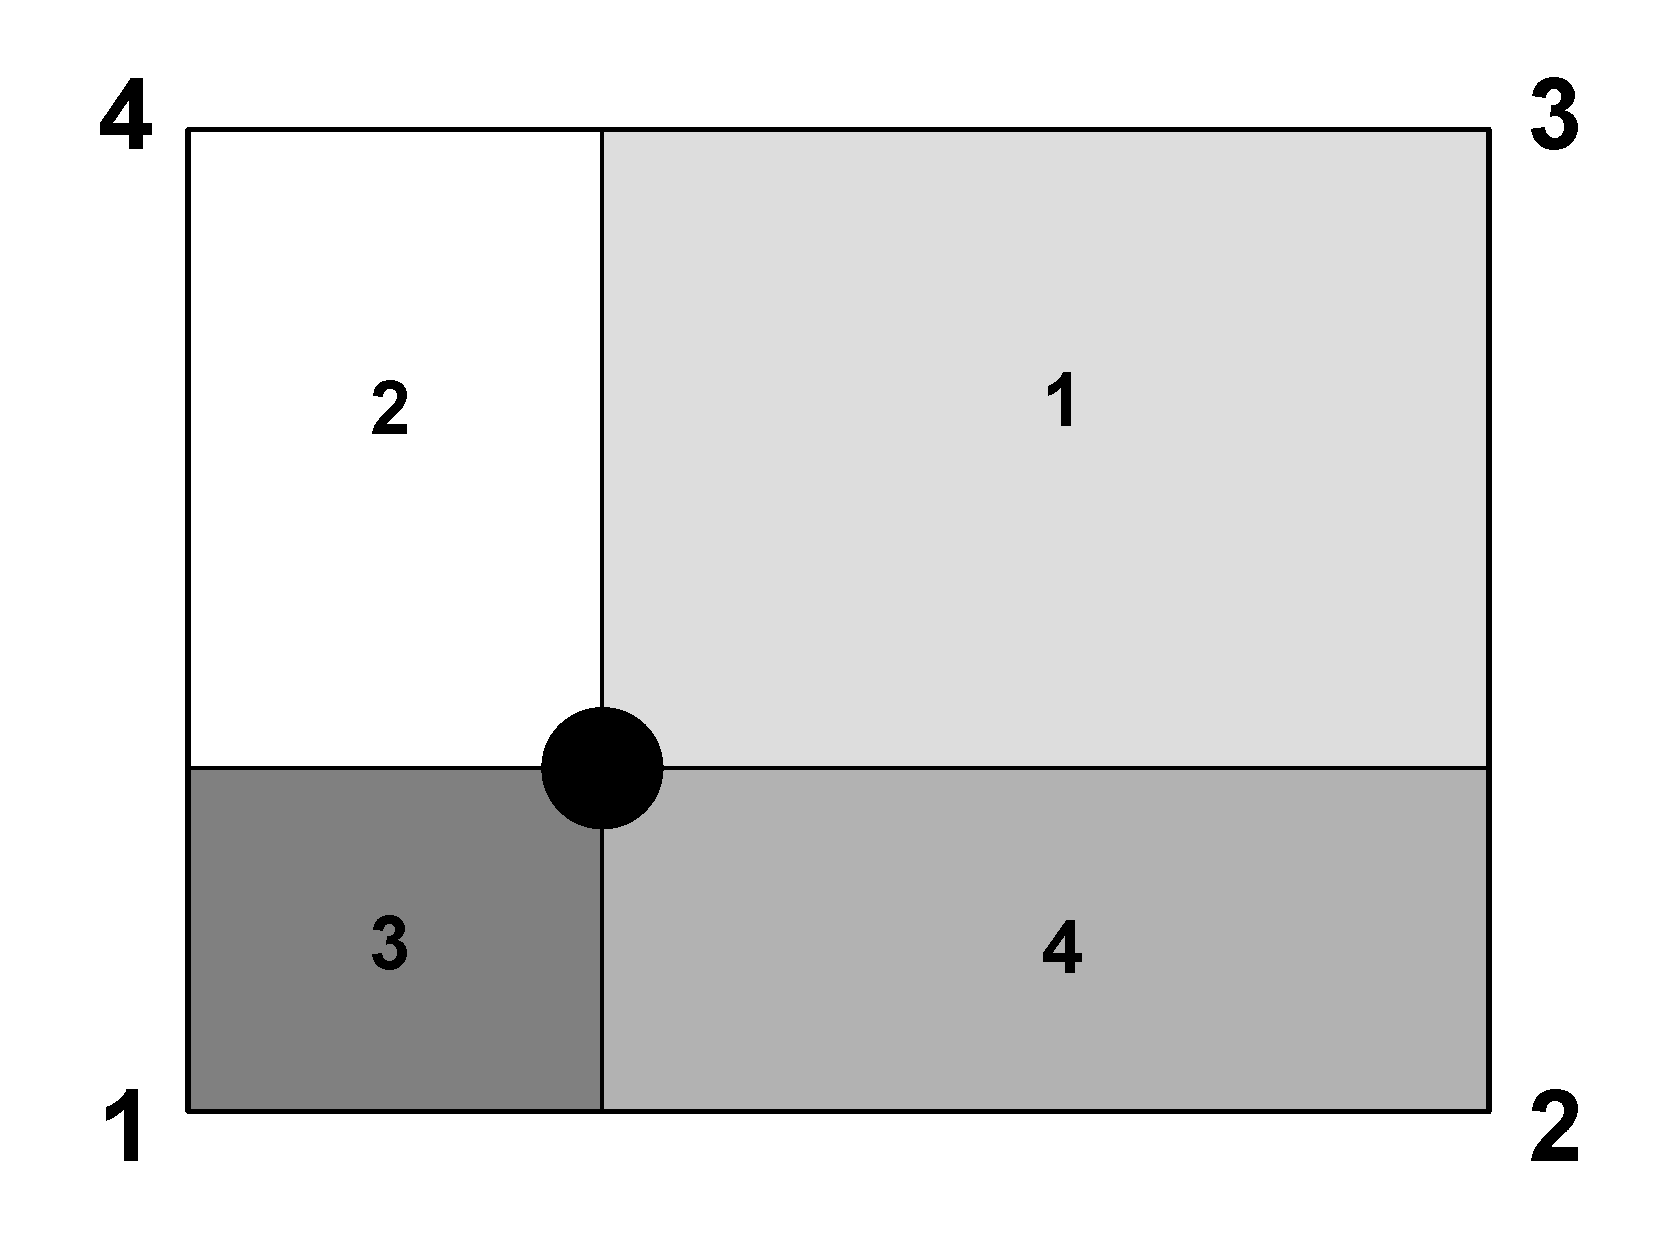
\includegraphics[width=8cm]{figures/1-03_pnn.pdf}
\caption{
Projection onto neighbouring nodes (PNN; simplified illustration for 2D case).
The contribution of the particle momentum to the fluid momentum at a grid node depends on the separation distance.
For example, the particle force may be projected onto neighbouring nodes using weights that are proportional to cell areas (or volumes in 3D case).
Here, the fluid flow at grid node $1$ is affected by a fraction of the particle Stokes drag proportional to the area with marker $1$, and so on.
Based on \textcite[Fig. 1 therein]{Garg2007}.}
\label{fig:pnn}
\end{figure}

\medskip

The total number of particles, $N_{\text{part}}$, is another parameter, besides grid size $N$, that mainly determines computational burden of simulations.
In this study, highest number of individually tracked particles was $20$ million and for droplets with smaller radii that was still not sufficient to achieve higher values of the mass loading.
Still, simulations with larger mass loading ($0.1 < \Phi_{m} < 1$) are necessary to clearly observe effects of two-way momentum coupling on measured statistics.
For that reason, in some simulations, super-particle parameterisation was used to increase $\Phi_m$ without adding new computational particles \parencite{Elghobashi1994}.
That parameterisation is applied by using weighting factor, $M$, in Equation \ref{eqn:twc-th}.
When $M=1$ each computational particle represents exactly one dropletand no extra parameterisation is involved.
For $M > 1$, however, every computational particle models a cluster of $M$ droplets (i.e. the super-particle) that is tracked together as a single point-particle with inflated mass by the factor of $M$.

Such parameterisation was used in \textcite{Rosa2020} for similar reasons and it was observed that it does not significantly affect measured collision statistics as long as $M$ is not too large.
Moreover, it was noted that these discrepancies are relatively small when mass loading is large, this is probably due to the stronger turbulence attenuation in simulations without gravity (turbulence is the main mechanism enforcing particle clustering).
On the other hand, in simulations with gravity a larger mass loading results in the formation of new vortical structures which cause the decorrelation of particle motion and consequently a more uniform spatial distribution.
More systematic analysis of the impact of this parameterisation was conducted in a recent study by \textcite{Rosa2022} where collision statistics from simulations with varying $M$ and fixed mass loading, $\Phi_m$, were analysed.
The clear tendency for that parameterisation to overestimate the radial relative velocity and underestimate the radial distribution function was reported.
For values of $M < 20$ the influence of super-particle parameterisation may be acceptable, but otherwise discrepancies rapidly cumulate and render obtained results applicable for only qualitative analysis at best (in some cases, for $M = 100$, values of RDF were halved, and for RRV inflated by the factor of $3$).
Moreover, even larger discrepancies were observed in simulations with gravity. 

Interestingly, some studies using more refined techniques of dealing with super-particles \parencite{Garg2009} have shown that errors arising from that parameterisation increase with refinement of the grid.
This may be beneficial when considering LES method, as it works on much coarser grid than comparable DNS.
Still, cumulative effects and possible interactions between these two parameterisations may be quite complex and hard to follow in a systematic and quantitative manner.



\section{Notes on Implementation}
\label{sc:ch1.impl}

The effective implementation of methods presented above is necessarily intended for massively parallel computation environments (supercomputers) due to large grids and particle populations that are required to produce physically meaningful results.
The solver code used in this study was long developed, tested, and improved upon to provide further capabilities \parencite[see~e.g.][]{Ayala2014,Parishani2015}, including modifications necessary to obtain results presented here.
It is implemented using Message Passing Interface (MPI) to facilitate communication between several processes executing the code.
The division of work is based on the concept of 2D domain decomposition where each process is handling all computations associated with one part (subdomain) of the entire computational domain.
In this case, the domain is divided along two out of three spatial axes into ''columns'' with equal number of grid nodes (see Figure \ref{fig:2dd}).
By default, two directions chosen for such decomposition are those orthogonal to the (vertical) direction of gravity, in order to minimise the number of particles crossing subdomain boundaries. 
This strategy is relatively simple to implement and quite efficient, at least if we assume that distribution of particles between subdomains is close to uniform (this assumption will be further analysed in Section \ref{sc:ch3.perfp}).
In this study, subdomains have dimensions $16 \times 16 \times N$ to provide large enough margin for convenient communication between processes.
In particular, for DNS and its grid with $256^{3}$ nodes we have $16^{2} = 256$ subdomains, and for LES with $64^{3}$ grid nodes -- $4^{2} = 16$ subdomains.
The number of processes used to execute solver code is equal to the number of subdomains used.

\begin{figure}[h]
\centering
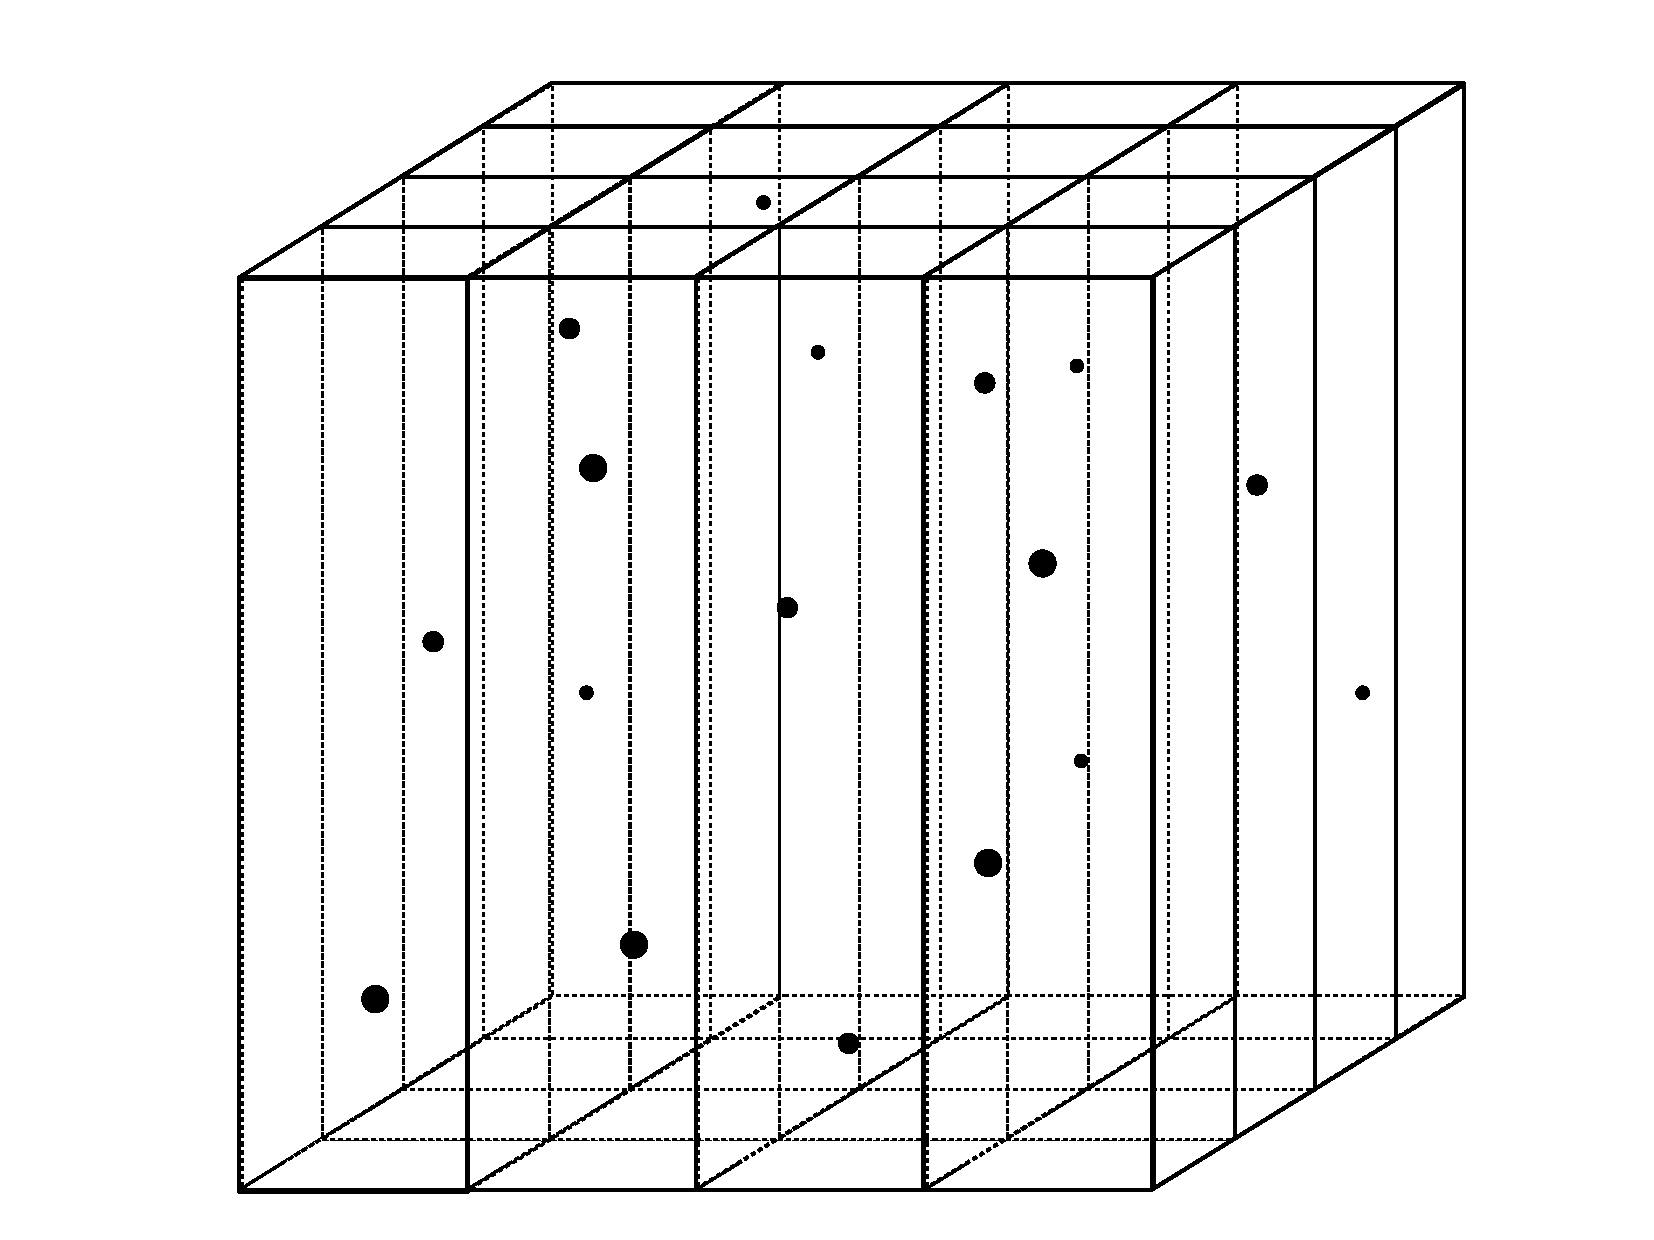
\includegraphics[width=10cm]{figures/1-04_2dd.pdf}
\caption{
Schematic representation of 2D domain decomposition.
This image corresponds to the actual decomposition of $64^{3}$ grid used for LES.
Entire domain is divided into $4 \times 4 = 16$ subdomains, each with $16 \times 16 \times 64$ nodes.
}
\label{fig:2dd}
\end{figure}

Exact steps that constitute each iteration of both DNS and LES method are summarised in Table \ref{tab:code-steps}.
In general, entire code may be divided into parts that handle computations involving either fluid flow or particle motion, as well as parts used for data postprocessing (i.e. to calculate and output interesting statistics of fluid flow and particles).
The heart of pseudo-spectral code is the efficient implementation of the fast Fourier transform, as every iteration requires performing 3D FFT three times.
Parallel implementation of 3D FFT is used as proposed by \textcite{Ayala2013}.
It is decomposed into three separate calls to 1D FFT procedures provided by \texttt{fftw} library together with an original procedure for data transposition.
The choice of 2D domain decomposition was mainly driven by the fact that it was found to be optimal for such implementation of parallel 3D FFT.  
It was chosen above 1D decomposition that was initially proposed by \textcite{Dmitruk2001}, since it heavily restricted number of parallel processes allowed to execute the code, and above 3D decomposition which introduced excessive costs of communication and data transfer between larger number of subdomains \parencite{Ayala2013}.   
The architecture used to store particle data and transfer it between processes is a key part of the implementation, as detection of nearby particles is crucial for efficient calculation of two-point particle collision statistics.
For that reason the concept of linked lists together with the cell-index method was employed according to \textcite[p. 149--152]{Allen1987}.
In every run statistics of the fluid flow and particles statistics are gathered only after the entire system has reached the statistically stationary state, which is not earlier than after approximately $10 T_e$ \parencite{Rosa2017}, where $T_e$ is turnover time for largest resolved eddies.  



\chapter{Physical Fidelity of DNS and LES Results}
\label{ch:ch2}

NNN



\chapter{Comparison of DNS and LES Performance}
\label{ch:ch3}

NNN



\chapter*{Conclusions}
\addcontentsline{toc}{chapter}{\numberline{}Conclusions}
\label{ch:end}

NNN


\appendix
\chapter{Pseudo-Spectral Method in Detail}
\label{app:psm}

NNN



\chapter{Effects of Subgrid-Scale Model on Flow Statistics}
\label{app:sgs}

NNN


\chapter{Super-Particle Parametrisations in Simulations under Two-Way Momentum Coupling}
\label{app:spp}

NNN


\addcontentsline{toc}{chapter}{\numberline{}References}
\printbibliography[title=References]

\end{document}
